We hope you have enjoyed \textit{Development Research in Practice: The DIME Analytics Data Handbook}.
Our aim was to teach you to handle data more efficiently, effectively, and ethically.
We laid out a complete vision of the tasks of a modern researcher,
from planning a project's data governance to publishing code and data
to accompany a research product.
We have tried to set the text up as a resource guide
so that you will always be able to return to it
as your work requires you to become progressively more familiar
with each of the topics included in the guide.

We started the book with a discussion of research as a public service:
one that requires you to be accountable to both research participants
and research consumers.
We then discussed the current research environment,
which necessitates cooperation with a diverse group of collaborators
using modern approaches to computing technology.
We outlined common research methods in impact evaluation,
with an eye toward structuring data work.
We discussed how to implement reproducible routines for sampling and randomization,
and to analyze statistical power and use randomization inference.
We discussed data collection
and analysis methods,
as well as tools and practices for making this work publicly accessible.
Throughout, we emphasized that data work is a ``social process'',
involving multiple team members with different roles and technical abilities.
This mindset and workflow, from top to bottom,
outline the tasks and responsibilities
that are fundamental to doing credible research.

However, as you probably noticed, the text itself provides
just enough detail to get you started:
an understanding of the purpose and function of each of the core research steps.
The references and resources get into the details
of how you will realistically implement these tasks:
from DIME Wiki pages detail specific code conventions
and field procedures that our team considers best practices,
to the theoretical papers that will help you figure out
how to handle the unique cases you will undoubtedly encounter.
We hope you will keep the book on your desk
(or the PDF on your desktop)
and come back to it anytime you need more information.
We wish you all the best in your work
and will love to hear any input you have on ours!\sidenote{
You can share your comments and suggestion on this book through \url{https://worldbank.github.io/dime-data-handbook}.}

\vspace{1cm}
\begin{fullwidth}
	\begin{figure}
		\centering
		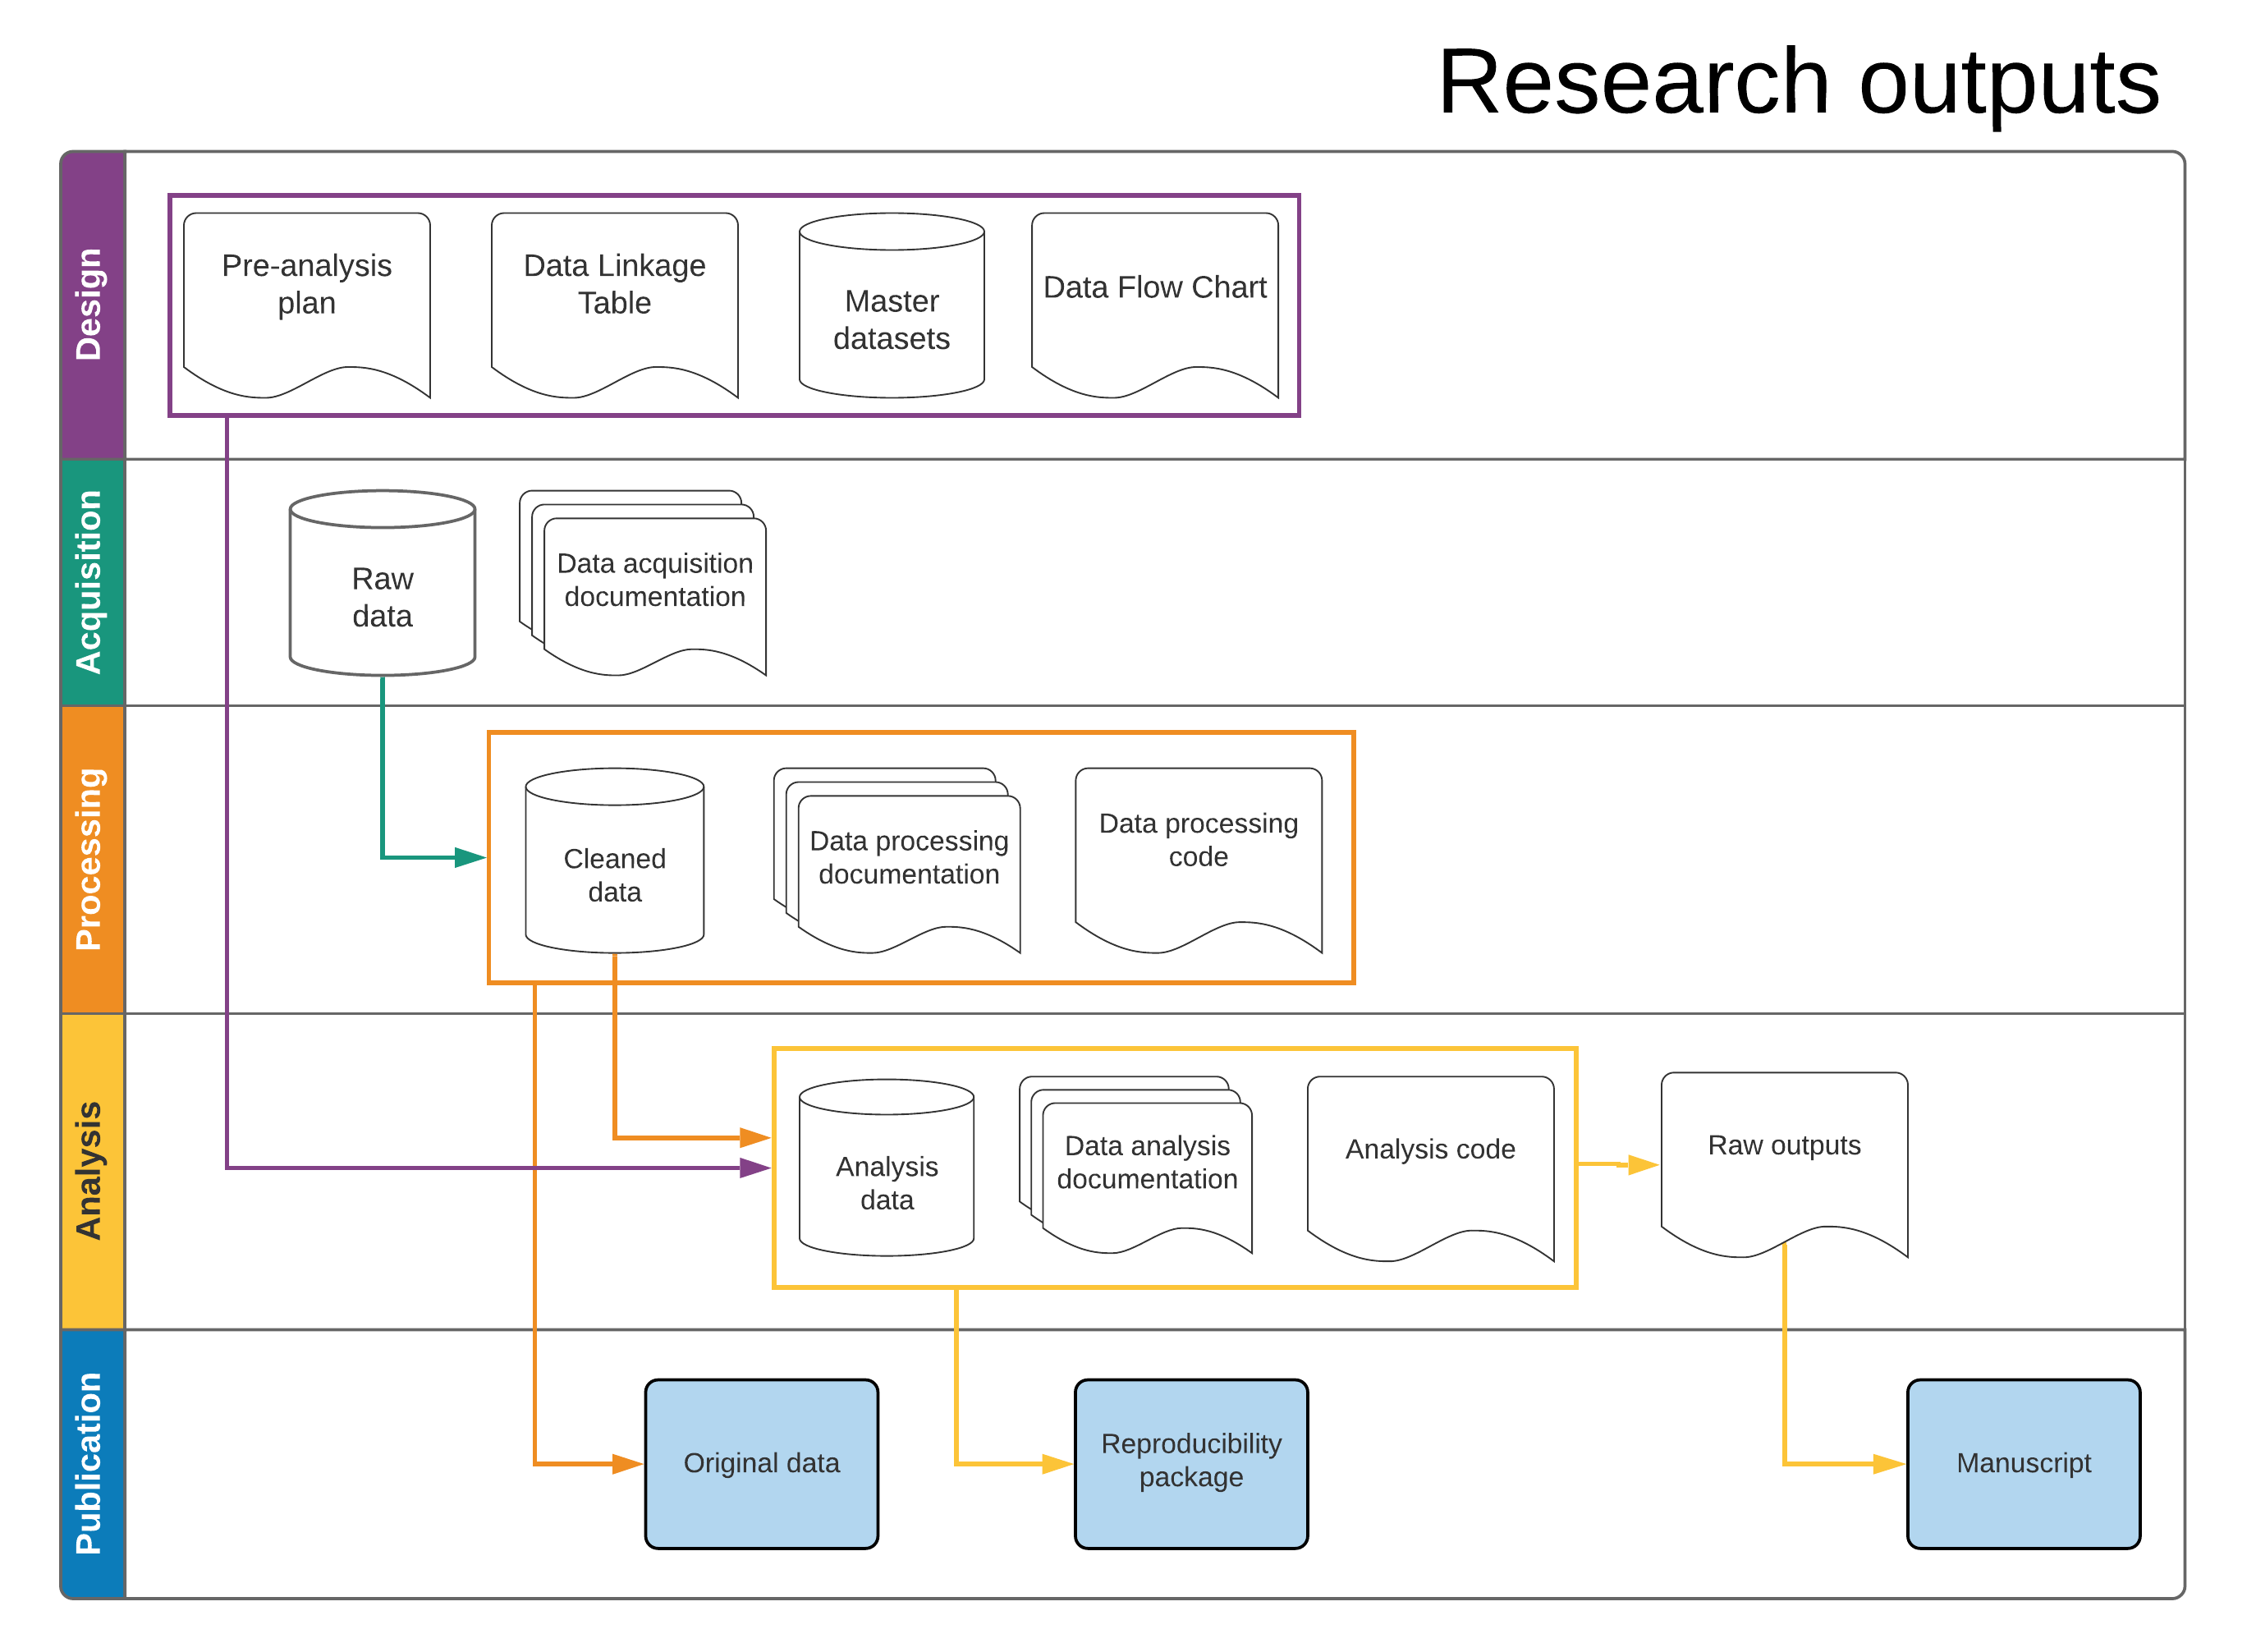
\includegraphics[width=1.6\linewidth]{diagrams/Conclusion}
		\caption{}
		\label{fig:intro}
	\end{figure}
\end{fullwidth}
